\subsection{Überprüfung der Stabilität}
Zur Überprüfung der Stabilitätsbedingung \eqref{eq:Stabilitat} werden die Messwerte normiert, sodass die höchste Intensität jeweils den Wert 1 zugewiesen bekommt. Die resultierenden, sowie die gemessenen Werte sind in den Tabellen VERWEIS und VERWEIS zu sehen. Dann wird für den Resonator mit den beiden konkaven Spiegeln ein quadratisches Polynom -- in Anlehnung an \eqref{eq:StabCurv} -- an die Messwerte für die normierten Intensitäten gefittet. Das Ergebnis ist in Abbildung \ref{fig:fitcurved} dargestellt. Dasselbe wird mit den Werten für den Resonator mit einem flachen Spiegel und einer linearen Funktion gemacht. Die Ergebnisse hierfür finden sich in Abbildung \ref{fig:fitflat}. Auf die Angabe der errechneten Parameter wird hier verzichtet, da die gefittete Funktion offensichtlich weit von den Erwartungen abweicht.
\begin{figure}[h!]
	\centering
	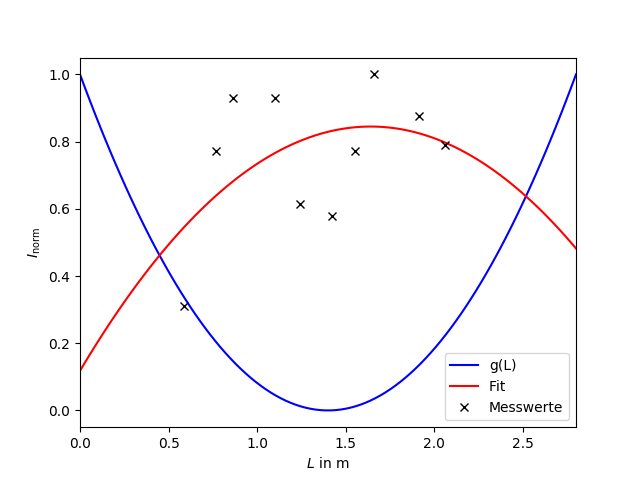
\includegraphics[width=.6\textwidth]{FitCurved.png}
	\caption{Fit zur Überprüfung der Stabilitätsbedingung bei zwei konkaven Spiegeln mit den Messwerten und der theoretisch erwarteten Funktion $g(L)$}
	\label{fig:fitcurved}
\end{figure}
\begin{figure}[h!]
	\centering
	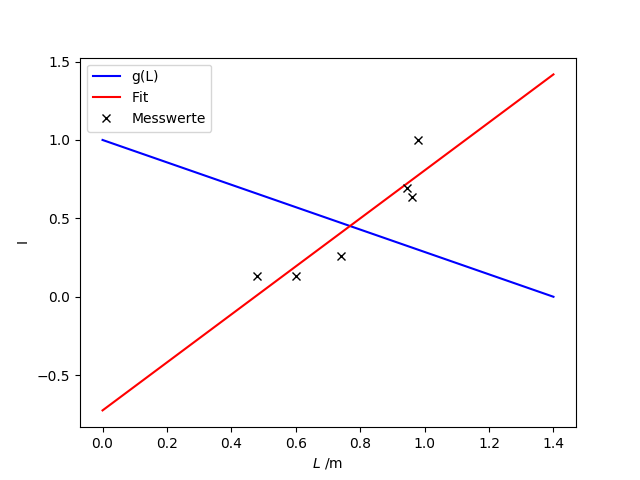
\includegraphics[width=.6\textwidth]{FitFlat.png}
	\caption{Fit zur Überprüfung der Stabilitätsbedingung bei einem gekrümmten und einem flachen Spiegel mit den Messwerten und der theoretisch erwarteten Funktion $g(L)$}
	\label{fig:fitflat}
\end{figure}